\chapter{Praktická časť}

Praktická časť práce opisuje návrh, implementáciu a overenie rozšírenia \textit{Toxic Text Detector}. Nadväzuje na analytickú časť, v ktorej boli predstavené teoretické východiská, existujúce prístupy k detekcii toxicity a technické požiadavky na riešenie v prostredí webového prehliadača. V tejto kapitole sú tieto poznatky pretavené do konkrétneho návrhu architektúry, používateľského rozhrania a implementácie jednotlivých komponentov systému.


\section{Úvod do praktickej časti}
Na základe poznatkov z analytickej časti a formulovaných cieľov práce bolo navrhnuté a implementované rozšírenie prehliadača na detekciu toxického textu. Praktická časť práce opisuje celý proces tvorby riešenia: od požiadaviek, návrhu architektúry a používateľského rozhrania až po implementáciu jednotlivých komponentov, lokálnu inferenciu, vzdialený režim cez API a návrh testovania.

Navrhované riešenie vychádza z požiadavky vytvoriť rozšírenie prehliadača založené na Chrome Manifest V3, ktoré dokáže analyzovať text priamo na webovej stránke, poskytnúť používateľovi zrozumiteľný výsledok klasifikácie a zároveň rešpektovať požiadavky na súkromie, bezpečnosť a použiteľnosť. Riešenie preto kombinuje lokálne spracovanie textu, možnosť vzdialenej inferencie a používateľské rozhranie umožňujúce jednoduchú konfiguráciu správania doplnku.

Cieľom tejto kapitoly je ukázať, ako boli teoretické poznatky pretavené do konkrétneho praktického riešenia. Kapitola najskôr definuje požiadavky a návrh architektúry, následne opisuje návrh a prototypovanie používateľského rozhrania a v ďalších častiach sa venuje samotnej implementácii rozšírenia \textit{Toxic Text Detector}.

\section{Požiadavky na riešenie}
Pred návrhom architektúry bolo potrebné určiť základné funkčné a nefunkčné požiadavky systému. Tieto požiadavky vychádzajú zo zadania práce, z analytickej časti a z očakávaného spôsobu používania rozšírenia pri prehliadaní webových stránok a online diskusií.

\subsection{Funkčné požiadavky}
Navrhované riešenie musí umožniť:
\begin{itemize}
  \item analyzovať text vybraný používateľom na podporovanej webovej stránke,
  \item automaticky identifikovať textové úseky, ktoré môžu byť toxické, ak je zapnutá funkcia automatickej ochrany,
  \item zobraziť výsledok klasifikácie vo forme hlavného verdiktu a skóre pre jednotlivé kategórie toxicity,
  \item prepínať medzi lokálnym a vzdialeným režimom inferencie,
  \item umožniť používateľovi meniť prísnosť detekcie a aktivovať alebo deaktivovať vybrané kategórie toxicity,
  \item uchovávať používateľské nastavenia medzi reláciami prehliadania,
  \item skryť a opätovne odhaliť označený obsah bez trvalého zásahu do štruktúry stránky.
\end{itemize}

\subsection{Nefunkčné požiadavky}
Okrem samotnej funkčnosti musí systém spĺňať aj nefunkčné požiadavky:
\begin{itemize}
  \item \textbf{Súkromie:} systém má prednostne spracúvať text lokálne a odosielať ho mimo zariadenia len v prípade povoleného vzdialeného režimu.
  \item \textbf{Bezpečnosť:} rozšírenie musí rešpektovať pravidlá Chrome Manifest V3 a nesmie ukladať citlivé API kľúče v klientskom kóde.
  \item \textbf{Odozva:} klasifikácia má prebiehať tak, aby výrazne nenarúšala čítanie stránky.
  \item \textbf{Zrozumiteľnosť:} používateľské rozhranie má jasne zobrazovať, čo bolo detegované a aký typ toxicity bol vyhodnotený.
  \item \textbf{Rozšíriteľnosť:} architektúra má umožniť neskoršie doplnenie ďalších modelov, kategórií alebo jazykových režimov.
\end{itemize}

\section{Návrh riešenia}
Navrhované riešenie je koncipované ako ochranná vrstva medzi používateľom a webovým obsahom. Jeho cieľom nie je nahradiť moderovanie platforiem, ale poskytnúť používateľovi nástroj, ktorý mu pomôže identifikovať potenciálne škodlivý obsah a rozhodnúť sa, či ho chce zobraziť.

Z konceptuálneho hľadiska systém pozostáva zo štyroch hlavných vrstiev:
\begin{enumerate}
  \item \textbf{Vrstva interakcie s používateľom,} ktorá zabezpečuje zobrazenie stavu ochrany, výsledkov analýzy a konfiguračných možností.
  \item \textbf{Vrstva spracovania webového obsahu,} ktorá pracuje s DOM štruktúrou stránky, identifikuje relevantné textové úseky a pripravuje ich na analýzu.
  \item \textbf{Vrstva inferencie,} ktorá vykonáva klasifikáciu textu lokálne alebo prostredníctvom vzdialeného API.
  \item \textbf{Vrstva konfigurácie a perzistencie,} ktorá uchováva používateľské nastavenia, aktívne kategórie a stav rozšírenia.
\end{enumerate}

Takéto rozdelenie oddeľuje zodpovednosti jednotlivých častí systému. Používateľské rozhranie sa stará o interakciu, obsahový skript o prácu so stránkou, inferenčná vrstva o vyhodnotenie textu a konfiguračná vrstva o stabilné uchovanie nastavení. Výhodou tohto prístupu je jednoduchšia údržba a možnosť meniť jednotlivé časti systému nezávisle od ostatných.

Vzťahy medzi používateľom, rozhraním, detekčným modulom a výsledkom klasifikácie sú znázornené na obrázku~\ref{fig:conceptual_model_ttd}. Model ukazuje, že používateľ nekomunikuje priamo s detekčným modelom, ale cez rozhranie rozšírenia. UI vrstva prijíma používateľské akcie, zobrazuje výsledok klasifikácie a sprostredkúva konfiguráciu správania rozšírenia. Detekčný modul spracúva text podľa aktuálnych nastavení a vracia jednotný výsledok obsahujúci celkový verdikt a skóre jednotlivých kategórií.

\begin{figure}[htbp]
  \centering
  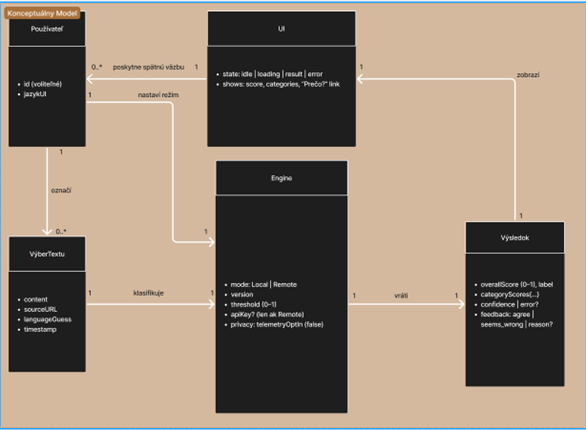
\includegraphics[width=0.82\linewidth,height=0.50\textheight,keepaspectratio]{figures/Konceptual}
  \caption{Konceptuálny model rozšírenia.}
  \label{fig:conceptual_model_ttd}
\end{figure}

Tento konceptuálny model bol použitý ako základ pre návrh architektúry, používateľského rozhrania a toku dát medzi jednotlivými časťami rozšírenia.

\subsection{Architektúra rozšírenia}
Architektúra riešenia vychádza z modelu rozšírení Chrome Manifest V3. Tento model prirodzene rozdeľuje funkcionalitu medzi content script, service worker a používateľské rozhranie rozšírenia. Každá z týchto častí má jasne definovanú úlohu.

\subsubsection{Content script}
Content script je komponent vložený do webovej stránky. V navrhovanom riešení zabezpečuje najmä:
\begin{itemize}
  \item získanie textu vybraného používateľom,
  \item výber textových blokov vhodných na automatickú analýzu,
  \item odoslanie textu na klasifikáciu,
  \item prijatie výsledkov inferencie,
  \item vizuálne označenie alebo rozmazanie toxického obsahu.
\end{itemize}

Content script musí byť navrhnutý tak, aby zbytočne nezaťažoval stránku. Pri automatickom skenovaní preto nemá analyzovať celý DOM bez obmedzení, ale iba vhodné textové prvky spĺňajúce dĺžkové a viditeľnostné kritériá.

\subsubsection{Service worker}
Service worker predstavuje koordinačný prvok rozšírenia. V prostredí Manifest V3 nahrádza pôvodné trvalé background pages a pracuje udalostne. V návrhu zabezpečuje:
\begin{itemize}
  \item prijímanie požiadaviek od používateľského rozhrania a content scriptu,
  \item rozhodovanie o použití lokálneho alebo vzdialeného režimu,
  \item sprostredkovanie komunikácie medzi komponentmi,
  \item vyvolanie opätovného skenovania stránky po zmene nastavení,
  \item správu akcií dostupných cez kontextové menu rozšírenia.
\end{itemize}

Keďže service worker nemá priamy prístup k DOM stránke, všetky operácie nad webovým obsahom musia byť delegované na content script. Tým sa zachováva bezpečnostný model rozšírenia a zároveň sa jasne oddeľuje práca so stránkou od globálnej logiky doplnku.

\subsubsection{Používateľské rozhranie}
Používateľské rozhranie je navrhnuté ako kombinácia rýchleho popup okna, obrazovky nastavení a prekrytia priamo na stránke. Popup slúži na rýchle zobrazenie stavu ochrany, počtu detegovaných prvkov a základných akcií. Obrazovka nastavení poskytuje priestor na podrobnejšiu konfiguráciu, napríklad výber aktívnych kategórií, prísnosti detekcie, režimu inferencie alebo whitelistu domén. Prekrytie na stránke umožňuje pracovať priamo s označeným obsahom.

\subsection{Návrh režimov inferencie}
Jedným z hlavných návrhových rozhodnutí je podpora dvoch režimov inferencie: lokálneho a vzdialeného. Tento hybridný prístup umožňuje vyvážiť požiadavky na súkromie, kvalitu klasifikácie a technickú realizovateľnosť.

\subsubsection{Lokálny režim}
V lokálnom režime prebieha klasifikácia priamo v prehliadači používateľa. Model je súčasťou rozšírenia alebo je načítaný ako jeho lokálny artefakt. Text preto nie je potrebné odosielať na externý server.

Výhodou lokálneho režimu je vyššia úroveň súkromia, nezávislosť od vzdialenej služby a rýchla odozva pri použití optimalizovaného modelu priamo v prehliadači. Nevýhodou je nižšia klasifikačná presnosť v porovnaní s výkonnejším vzdialeným modelom, najmä pri menej zastúpených kategóriách.

\subsubsection{Vzdialený režim}
Vo vzdialenom režime rozšírenie odošle text na vlastný backend alebo proxy API, ktoré zabezpečí klasifikáciu pomocou vzdialeného modelu. Tento režim je vhodný v prípadoch, keď je potrebná vyššia presnosť alebo jednoduchšie experimentovanie s rôznymi modelmi bez nutnosti meniť klientsku časť rozšírenia. Rýchlosť vzdialeného režimu závisí od konkrétneho nasadenia backendu, použitého hardvéru, veľkosti modelu a sieťovej latencie. V testovanom prostredí bolo API spustené lokálne na výkonnom notebooku, preto bola odozva vzdialeného režimu blízka lokálnemu režimu.

Proxy vrstva zároveň chráni citlivé údaje, pretože API kľúče nie sú uložené v klientskom kóde rozšírenia. Okrem toho môže zabezpečiť jednotný formát odpovede, obmedzenie dĺžky vstupu, limitovanie požiadaviek a meranie latencie.

\subsubsection{Prepínanie medzi režimami}
Prepínanie medzi režimami môže byť realizované manuálne používateľom v nastaveniach alebo podmienene podľa jazyka a dostupnosti lokálneho modelu. Z návrhového hľadiska je vhodné, aby bol lokálny režim predvolený a vzdialený režim sa použil len vtedy, keď ho používateľ povolí alebo keď je potrebný pre konkrétny scenár.

Takýto prístup podporuje zásadu \textit{privacy-by-default}, pretože text sa mimo zariadenia neposiela automaticky bez jasnej potreby alebo nastavenia používateľom.

\subsection{Návrh toku dát}
Spracovanie textu v rozšírení prebieha ako postupnosť krokov medzi používateľským rozhraním, content scriptom, service workerom a inferenčnou vrstvou.

Typický scenár manuálnej kontroly vybraného textu pozostáva z nasledujúcich krokov:
\begin{enumerate}
  \item Používateľ označí text na webovej stránke.
  \item Content script získa označený text a pripraví požiadavku na analýzu.
  \item Požiadavka sa odošle príslušnej časti rozšírenia podľa zvoleného režimu.
  \item Inferenčná vrstva vykoná klasifikáciu textu.
  \item Výsledok sa vráti späť content scriptu.
  \item Content script zobrazí výsledok alebo vizuálne označí analyzovaný text.
\end{enumerate}

Pri automatickom skenovaní stránky je proces podobný, ale namiesto jedného vybraného textu sa pracuje s množinou textových úsekov. Aby sa znížila záťaž stránky, návrh počíta s obmedzením počtu analyzovaných prvkov, dávkovým spracovaním, cache výsledkov a filtrovaním nerelevantných DOM prvkov.

\subsection{Návrh práce s kategóriami toxicity a prahmi}
Keďže detekcia toxicity je problém viacnásobnej klasifikácie, systém nemá poskytovať iba jedno binárne rozhodnutie. Každý analyzovaný text môže patriť do viacerých kategórií súčasne, napríklad všeobecná toxicita, urážka, obscénnosť, hrozba alebo nenávisť voči identite.

Výsledok klasifikácie by preto mal obsahovať:
\begin{itemize}
  \item hlavný verdikt, či ide o potenciálne toxický obsah,
  \item skóre pre jednotlivé kategórie,
  \item informáciu o tom, ktoré kategórie prekročili nastavené prahy,
  \item voliteľné upozornenie pri nižšej spoľahlivosti výsledku.
\end{itemize}

Prahy detekcie nemusia byť rovnaké pre všetky kategórie. Napríklad hrozby môžu vyžadovať citlivejší prah než všeobecná toxicita. Preto návrh počíta s internými prahmi pre jednotlivé kategórie a s používateľským nastavením prísnosti, ktoré tieto prahy upravuje jednoduchým a zrozumiteľným spôsobom.

\subsection{Bezpečnostné a súkromnostné opatrenia}
Bezpečnosť a ochrana súkromia patria medzi hlavné kritériá návrhu. Systém preto uplatňuje tieto zásady:
\begin{itemize}
  \item lokálne spracovanie je preferovaný režim,
  \item vzdialené spracovanie je používateľovi zreteľne signalizované,
  \item API kľúče sa neukladajú v klientskom kóde,
  \item rozšírenie nepoužíva vzdialene hostovaný vykonateľný kód,
  \item analyzujú sa iba relevantné textové časti stránky,
  \item uchováva sa len nevyhnutné minimum nastavení a spätnej väzby.
\end{itemize}

Takýto návrh je v súlade s technickými obmedzeniami Manifest V3 a zároveň podporuje princípy minimalizácie údajov a transparentnosti voči používateľovi.

\section{Prototypovanie používateľského rozhrania}
Používateľské rozhranie doplnku \textit{Toxic Text Detector} bolo navrhované iteratívne formou prototypovania v dvoch hlavných iteráciách. Cieľom rozhrania bolo umožniť používateľovi rýchlo rozpoznať potenciálne toxické časti online diskusií, pričom zásah do čítania mal zostať čo najmenší. Dôležitou požiadavkou bola aj reverzibilita akcií, pretože používateľ musí mať možnosť označený text kedykoľvek zobraziť alebo opätovne skryť.

Prvá iterácia vznikla ako interaktívny prototyp vo Figme. Slúžila najmä na overenie rozloženia obrazoviek, pomenovania prvkov a základných interakčných vzorov, ako je rozmazanie toxického textu, odhalenie obsahu, otvorenie vysvetlenia a prístup k nastaveniam. Druhá iterácia bola vytvorená ako bežiaci HTML/React prototyp pomocou technológií Vite a React. Táto verzia už lepšie približovala správanie finálneho rozšírenia, najmä popup okno, stránku nastavení a prekrytie priamo na webovej stránke.

\subsection{UX výskum}
UX výskum sa zameral na situáciu, v ktorej používateľ prehliada verejné diskusie alebo dlhšie vlákna komentárov. V takomto prostredí je dôležité, aby ochrana nevyžadovala zložité rozhodovanie pri každom komentári. Používateľ má byť chránený pred nechceným obsahom, ale zároveň má mať možnosť zobraziť si text v prípade potreby, napríklad pri moderovaní alebo pri posudzovaní kontextu diskusie.

Z návrhového hľadiska boli sledované najmä tieto otázky:
\begin{itemize}
  \item Ako môže rozhranie signalizovať toxicitu bez zbytočného prerušenia čítania?
  \item Ako zachovať akcie reverzibilné, aby používateľ nestratil kontrolu nad obsahom?
  \item Aké minimum vysvetlenia je potrebné, aby používateľ výsledku detekcie rozumel?
  \item Ako sprístupniť nastavenia tak, aby boli dostupné, ale nie rušivé?
\end{itemize}

Na základe analýzy potrieb boli identifikované dve typické skupiny používateľov:
\begin{itemize}
  \item \textbf{Bežný používateľ:} chce rýchlo prehliadať diskusie bez zbytočných zásahov do čítania.
  \item \textbf{Moderátor alebo správca komunity:} potrebuje obsah zobraziť aj v prípade ochrany, no zároveň chce jasné označenie rizikových častí.
\end{itemize}

\subsection{Návrh sekvencií obrazoviek}
Návrh toku obrazoviek bol postavený okolo kontinuálnej slučky prehliadania:
\textit{čítať} $\rightarrow$ \textit{detegovať} $\rightarrow$ \textit{voliteľne odhaliť} $\rightarrow$ \textit{pochopiť dôvod} $\rightarrow$ \textit{upraviť nastavenia} $\rightarrow$ \textit{pokračovať v čítaní}.

Interakcia je ukotvená priamo v zozname komentárov, zatiaľ čo globálna konfigurácia je dostupná cez popup rozšírenia a obrazovku nastavení. Na zníženie interakčných nákladov používa UI rovnaký štrukturálny vzor naprieč obrazovkami: jasnú hlavičku, jednu primárnu obsahovú oblasť a obmedzenú množinu akcií.

Základné obrazovky a akcie sú znázornené na obrázku~\ref{fig:screen_sequence_proto2}. Tento návrh bol použitý ako podklad pre implementáciu bežiaceho HTML/React prototypu.

\begin{figure}[htbp]
  \centering
  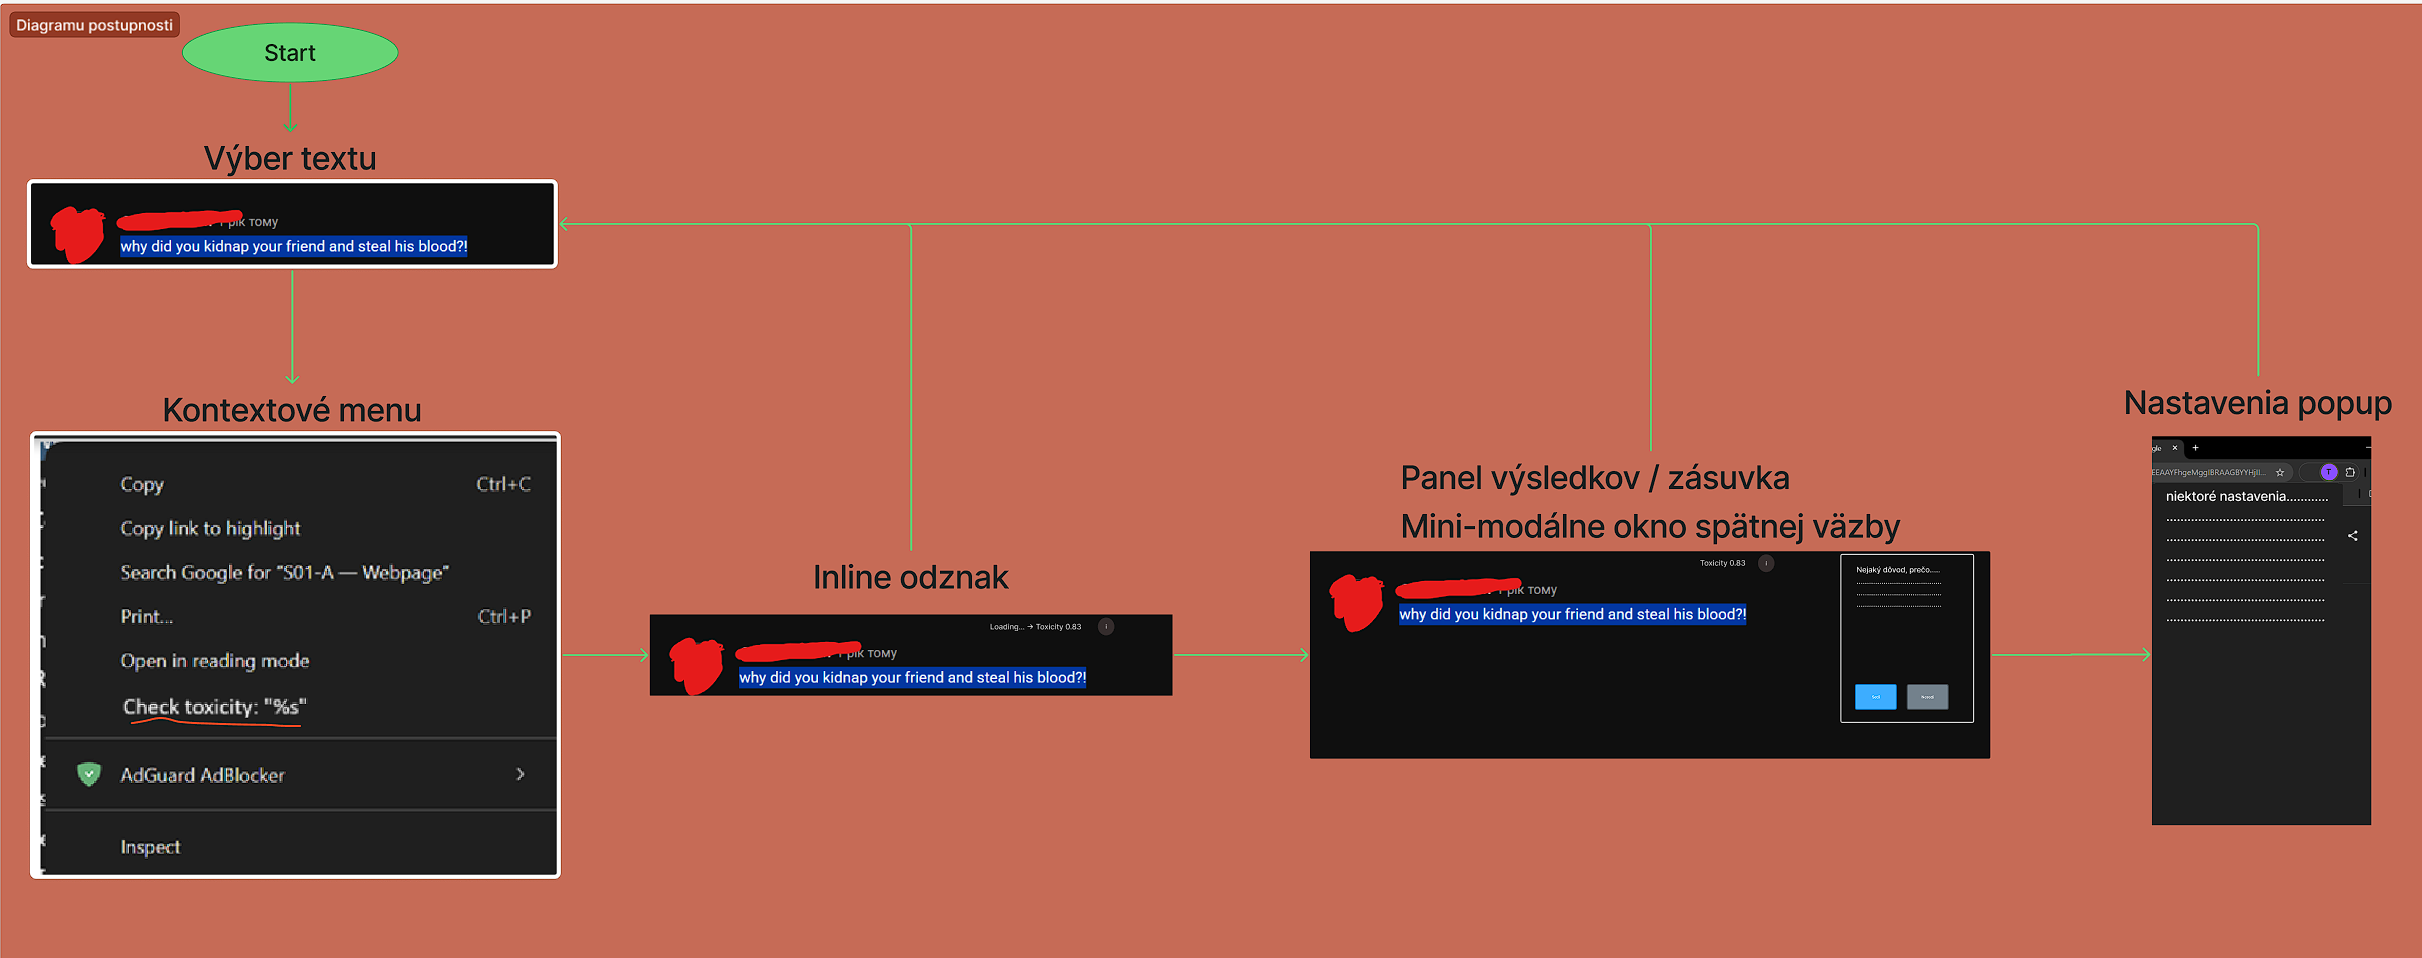
\includegraphics[width=0.90\linewidth,height=0.55\textheight,keepaspectratio]{figures/Sekv}
  \caption{Návrh postupností obrazoviek a navigácie rozšírenia.}
  \label{fig:screen_sequence_proto2}
\end{figure}

Navrhnuté boli najmä tieto časti používateľského rozhrania:
\begin{itemize}
  \item \textbf{Prekrytie na stránke:} toxické komentáre sú predvolene rozmazané, ak je zapnuté automatické rozmazanie.
  \item \textbf{Ovládanie na úrovni komentára:} používateľ môže text zobraziť alebo skryť a otvoriť vysvetlenie dôvodu označenia.
  \item \textbf{Popup rozšírenia:} zobrazuje stav ochrany, počet aktívnych kategórií a základné metriky aktivity.
  \item \textbf{Nastavenia:} umožňujú zapnúť alebo vypnúť kategórie, upraviť prísnosť detekcie a spravovať whitelist domén.
\end{itemize}

\subsection{Prototypy používateľského rozhrania}
Prvý prototyp bol vytvorený vo Figme ako interaktívny mock-up so strednou vernosťou. Jeho cieľom bolo overiť mentálny model a základný interakčný vzor bez implementačných detailov, najmä rozmazanie toxického textu, zobrazenie a skrytie na úrovni komentára, prístup k nastaveniam a jednoduché mini-modálne okno spätnej väzby. Mini-modálne okno spätnej väzby zostalo iba súčasťou skorého návrhu používateľského rozhrania. Do finálnej implementácie rozšírenia nebolo zahrnuté, pretože prvé riešenie nepôsobilo dostatočne použiteľne a jeho dopracovanie by si vyžadovalo samostatný návrh, ukladanie dát a ďalšie testovanie.

\begin{figure}[htbp]
  \centering
  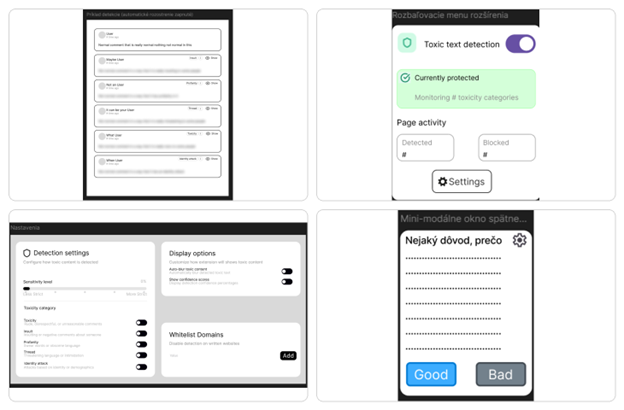
\includegraphics[width=0.90\linewidth,height=0.55\textheight,keepaspectratio]{figures/Prot1}
  \caption{Prvý prototyp vo Figme.}
  \label{fig:prototype1_figma}
\end{figure}

Druhý prototyp implementoval overený interakčný vzor v bežiacom HTML/React prototype. Táto iterácia zvýšila fidelitu návrhu a zabezpečila, že všetky prepínače a stavy sa správajú konzistentne: globálne zapnutie ochrany, automatické rozmazanie, zapnutie a vypnutie kategórií a voliteľné zobrazenie confidence skóre. Stav bol centralizovaný cez kontext nastavení, aby popup, obrazovka nastavení a karty komentárov na stránke vždy reflektovali rovnakú konfiguráciu.

\begin{figure}[htbp]
  \centering
  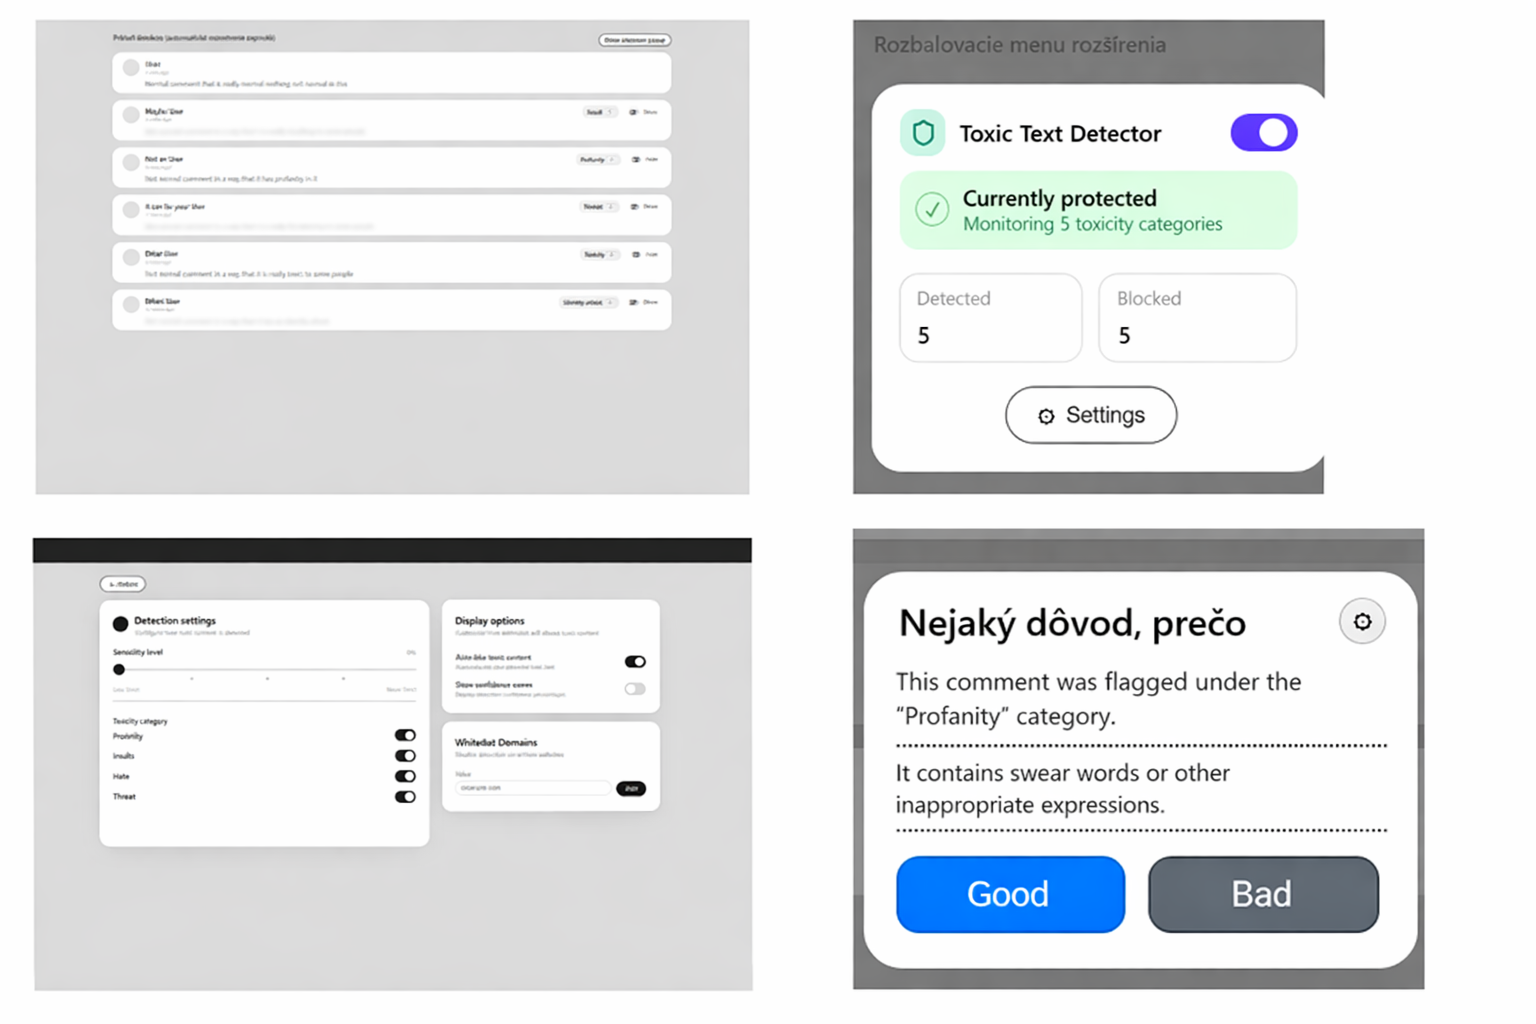
\includegraphics[width=0.90\linewidth,height=0.55\textheight,keepaspectratio]{figures/Prot2}
  \caption{Ukážka implementovaného rozhrania v druhom prototype.}
  \label{fig:prototype2_react}
\end{figure}

Pre potreby dokumentácie sú uvedené aj odkazy na zdroje návrhu:
\begin{itemize}
  \item Zdrojový súbor prototypu: \href{https://www.figma.com/design/To6xEq40ptUYcN36ClJxXR/UX-2-Stakhov-Vladysav?node-id=0-1&t=iu2xqZT8ewasfSXn-1}{Figma Design File}.
  \item Interaktívny náhľad prototypu: \href{https://www.figma.com/design/To6xEq40ptUYcN36ClJxXR/UX-2-Stakhov-Vladysav?node-id=0-1&t=iu2xqZT8ewasfSXn-1}{Figma Prototype}.
  \item Detailný popis, testovacie scenáre a výsledky: \href{https://www.figma.com/board/uDsfPT4P9LXAWeYCLPSIT0/UX-3-Stakhov-Vladysav?node-id=0-1&p=f&t=pL4GL526mWDMBFQd-0}{FigJam -- Prototypovanie a testovanie}.
\end{itemize}

\subsection{Zmeny na základe prototypovania}
Na základe priebežných zistení počas návrhu boli realizované tieto kľúčové zmeny:
\begin{itemize}
  \item \textbf{Zlepšenie vizuálnej hierarchie v kartách komentárov:} zvýraznenie hlavičky a zníženie vizuálnej dominance sekundárnych informácií.
  \item \textbf{Presun kontextových akcií do hlavičky karty:} rýchlejšia objaviteľnosť ovládania, napríklad reveal/hide a vysvetlenia dôvodu označenia.
  \item \textbf{Funkčné prepínače kategórií:} vypnutie kategórie okamžite upraví správanie detekcie a rozmazania pre daný typ toxicity.
  \item \textbf{Zjednotenie stavov v celom UI:} popup, nastavenia a prekrytie na stránke vždy zobrazujú tú istú konfiguráciu.
  \item \textbf{Jasnejší systém stavov:} chránený stav využíva výraznejšiu status kartu, zatiaľ čo vypnutý stav používa neutrálnejší vizuál.
\end{itemize}

Kompletný zdrojový kód prototypu je dostupný v repozitári:
\begin{itemize}
  \item \textbf{GIT projekt:} \href{https://git.kpi.fei.tuke.sk/vs800ru/ux3-vladyslav-stakhov}{git.kpi.fei.tuke.sk}.
\end{itemize}

\section{Implementácia rozšírenia}
Výsledná implementácia rozšírenia \textit{Toxic Text Detector} pozostáva zo štyroch hlavných častí: konfiguračnej vrstvy rozšírenia, používateľského rozhrania vytvoreného v Reacte, background logiky vo forme service workera a content scriptu, ktorý vykonáva lokálnu detekciu toxicity priamo na stránke.

Konfigurácia rozšírenia je definovaná v súbore \emph{manifest.json}. Použitý je formát Chrome Manifest V3, v ktorom je ako service worker zaregistrovaný súbor \emph{background.js}. Manifest zároveň určuje popup okno \emph{popup.html}, stránku nastavení \emph{options.html}, content scripty a web-accessible resources potrebné pre TensorFlow.js a WASM backend.

Používateľské rozhranie rozšírenia je implementované v priečinku \emph{src}. Popup rozhranie sa inicializuje cez súbor \emph{popupMain.jsx}, stránka nastavení cez \emph{optionsMain.jsx}. Obe časti používajú spoločný kontext \emph{SettingsContext.jsx}, ktorý zabezpečuje jednotnú prácu s nastaveniami a ich uloženie do synchronizovaného úložiska prehliadača.

Samotná lokálna detekcia toxicity je implementovaná v súbore \emph{contentScript.js}. Tento súbor obsahuje načítanie modelu, výber kandidátnych textových uzlov, klasifikáciu textu, prácu s cache a vizuálne označovanie toxického obsahu na stránke. Background skript \emph{background.js} vytvára kontextové menu a sprostredkúva komunikáciu medzi popup rozhraním a content scriptom aktívnej karty.

\subsection{Build proces a konfigurácia}
Build proces bol realizovaný pomocou nástroja Vite. Konfigurácia v súbore \emph{vite.config.js} definuje dva vstupné body: \emph{popup.html} a \emph{options.html}. Pri produkčnom zostavení sa tak generujú dve samostatné HTML stránky rozšírenia, pričom každá načítava svoj vlastný React vstupný bod.

Súbor \emph{popup.html} načítava skript \emph{popupMain.jsx}, zatiaľ čo \emph{options.html} načítava súbor \emph{optionsMain.jsx}. Popup rozhranie a stránka nastavení sa preto zostavujú nezávisle, ale stále používajú spoločné komponenty a zdieľaný stav.

Závislosti projektu sú definované v súbore \emph{package.json}. Pre používateľské rozhranie sú použité knižnice React a React DOM. Lokálna inferencia využíva TensorFlow.js, model Toxicity a WASM backend. Produkčný build sa vytvára príkazom \emph{npm run build}.

Manifest deklaruje používanie Manifest V3, service worker \emph{background.js}, popup okno rozšírenia, stránku nastavení, content scripty a web-accessible resources. V rámci content scriptov sa načítavajú knižnice pre jadro TensorFlow.js, konverziu modelu, backendy WASM a CPU, model \emph{toxicity.min.js}, pomocný kontrakt \emph{toxicityContract.global.js} a hlavná implementácia \emph{contentScript.js}. Web-accessible resources obsahujú najmä WASM súbory a priečinok s kernelmi, ktoré TensorFlow.js potrebuje pri lokálnom behu modelu.

\subsection{Implementácia popup rozhrania}
Popup rozhranie je inicializované v súbore \emph{popupMain.jsx}. Tento súbor vytvára React koreň, obalí popup komponent do \emph{SettingsProvider} a pomocou hooku \emph{useTabStats} priebežne načítava štatistiky z aktívnej karty.

Komponent \emph{PopupRoot} získava zo stavového kontextu informáciu o tom, či je rozšírenie zapnuté, a zároveň z hooku \emph{useTabStats} načítava počty detegovaných a zablokovaných prvkov. Po kliknutí na prepínač ochrany sa zavolá funkcia \emph{toggleEnabled()} a následne sa background skriptu odošle správa pre opätovné skenovanie aktívnej karty. Tým sa vyžiada nové skenovanie aktuálnej stránky.

Samotný vizuál popup okna je implementovaný v komponente \emph{ExtensionPopup.jsx}. Tento komponent prijíma všetky potrebné dáta cez props: stav ochrany, callback na jej prepnutie, callback na otvorenie nastavení, počet aktívnych kategórií a štatistiky z aktuálnej stránky. Popup zobrazuje hlavnú kartu so stavom ochrany, prepínač, dva informačné bloky s počtom detegovaných a blokovaných prvkov a tlačidlo pre otvorenie nastavení. Štýly popup okna sú definované v súbore \emph{popup.css}.

\subsection{Implementácia stránky nastavení}
Stránka nastavení sa inicializuje v súbore \emph{optionsMain.jsx}. Rovnako ako popup rozhranie používa \emph{SettingsProvider}, takže všetky zmeny nastavení sú zapisované do rovnakého dátového modelu.

Hlavným komponentom tejto časti je \emph{SettingsLayout.jsx}. Tento komponent používa hodnoty a funkcie zo súboru \emph{SettingsContext.jsx} a vykresľuje ich vo forme viacerých kariet rozdelených podľa typu nastavení. Implementácia obsahuje posuvník citlivosti detekcie, prepínače jednotlivých kategórií toxicity, prepínač automatického rozmazania toxického textu, prepínač zobrazenia confidence skóre, formulár pre pridanie domény do whitelistu, tlačidlo na reset nastavení, export a import nastavení vo formáte JSON a tlačidlo na manuálne opätovné skenovanie aktívnej karty.

Pri zmene citlivosti alebo pri prepnutí niektorej kategórie komponent okamžite volá funkciu \emph{pingRescan()}, ktorá odošle background skriptu správu pre opätovné skenovanie aktívnej karty. Takto sa zmena nastavenia okamžite prejaví aj na otvorenej stránke bez potreby ručného obnovenia karty. Štýly tejto časti sú definované v súbore \emph{settings.css}.

\subsection{Správa nastavení a perzistencia}
Zdieľaný stav rozšírenia je implementovaný v súbore \emph{SettingsContext.jsx}. Tento súbor definuje konštantu \emph{DEFAULT\_SETTINGS}, ktorá obsahuje predvolený stav ochrany, citlivosť, nastavenia zobrazenia, aktívne kategórie toxicity a whitelist domén.

Po inicializácii \emph{SettingsProvider} sa z úložiska načíta uložený objekt nastavení. Ak nastavenia v úložisku neexistujú, použijú sa predvolené hodnoty. Po každej zmene stavu sa aktualizovaná konfigurácia uloží späť.

Kontext zároveň poskytuje funkcie \emph{toggleEnabled()}, \emph{setSensitivity()}, \emph{toggleAutoBlur()}, \emph{toggleShowConfidence()}, \emph{toggleCategory()}, \emph{addWhitelist()} a \emph{removeWhitelist()}, ktoré používajú popup a stránka nastavení. Normalizácia domén je implementovaná pomocnou funkciou \emph{normalizeDomain()}, ktorá odstraňuje protokol, cestu a prefix \emph{www}. Táto funkcia sa používa pri ukladaní whitelistu, aby sa rôzne zápisy tej istej domény neukladali ako odlišné hodnoty.

\subsection{Background logika a komunikácia}
Service worker rozšírenia je implementovaný v súbore \emph{background.js}. Táto časť nepracuje s DOM stromom stránky, ale zabezpečuje centrálne akcie rozšírenia a komunikáciu s content scriptom.

Pri inštalácii a štarte rozšírenia sa vytvárajú tri položky kontextového menu: kontrola vybraného textu na toxicitu, skenovanie stránky na toxicitu a odstránenie existujúcich označení toxicity. Po kliknutí na niektorú z týchto položiek service worker vyhľadá aktívnu kartu a odošle jej správu cez rozhranie kariet, čím spustí príslušnú akciu v content scripte.

Background skript zároveň spracúva správy od popup rozhrania. Pri požiadavke na získanie štatistík najprv zistí aktívnu kartu a potom od content scriptu vyžiada štatistiky stránky. Pri požiadavke na opätovné skenovanie aktívnej karty odošle content scriptu správu na nové skenovanie stránky. Takto popup rozhranie získa údaje o stránke bez priameho prístupu k DOM.

Keďže background skript v MV3 nemá priamy prístup k obsahu stránky, všetky akcie nad obsahom musia byť delegované na content script. Tento model sa používa pri kontrole vybraného textu, pri skenovaní celej stránky aj pri odstraňovaní existujúcich označení.

\section{Implementácia lokálnej inferencie toxicity}

Táto časť sa venuje lokálnemu spracovaniu textu priamo v prostredí prehliadača. Opisuje načítanie modelu, normalizáciu výstupu, klasifikáciu textových úsekov, prácu s cache a spôsob vizuálneho označovania toxického obsahu na webovej stránke. Lokálna inferencia je dôležitou súčasťou riešenia, pretože podporuje ochranu súkromia používateľa a znižuje závislosť od vzdialených služieb.

\subsection{Načítanie modelu a normalizácia výstupu}
Lokálny model je načítavaný v content scripte funkciou \emph{loadToxicityModel()}. Implementácia používa premennú \emph{modelPromise}, aby sa model nenačítaval opakovane pri každej klasifikácii. Po prvom zavolaní sa vytvorený prísľub znovu používa pri ďalších požiadavkách.

Funkcia najprv nastaví cestu k WASM súboru pomocou rozhrania TensorFlow.js, pričom cesta sa generuje cez runtime API rozšírenia. Následne sa systém pokúsi aktivovať backend \emph{wasm}. Ak inicializácia zlyhá, použije sa fallback na backend \emph{cpu}.

Po úspešnej inicializácii backendu sa načíta model toxicity, pričom zoznam štítkov obsahuje kategórie \emph{toxicity}, \emph{severe toxicity}, \emph{obscene}, \emph{insult}, \emph{threat} a \emph{identity attack}. Prahová hodnota modelu je pri načítaní nastavená na nulovú hodnotu, pretože konečné rozhodovanie o toxicite sa nerobí priamo na úrovni predvoleného prahu modelu, ale cez vlastnú logiku implementovanú v súbore \emph{toxicityContract.global.js}.

Súbor \emph{toxicityContract.global.js} implementuje pomocnú vrstvu medzi surovým výstupom modelu a logikou rozšírenia. Definuje zoznam štítkov, základné prahové hodnoty, funkcie pre normalizáciu požiadavky, normalizáciu skóre, úpravu prahov podľa používateľskej prísnosti a výpočet finálneho verdiktu. Najdôležitejšou časťou je funkcia, ktorá z prijatých skóre vytvorí jednotný objekt odpovede obsahujúci režim detekcie, názov modelu, normalizované skóre, aplikované prahy, výsledný verdikt, spustené kategórie a latenciu klasifikácie.

Používateľské rozhranie pracuje s kategóriami \textit{Toxicity}, \textit{Insult}, \textit{Profanity}, \textit{Threat} a \textit{Identity attack}. Tieto kategórie sa v content scripte mapujú na konkrétne modelové štítky pomocou funkcie \emph{buildContractSettingsFromUI()}. Rovnako sa tu prevádza používateľská hodnota \emph{sensitivity} na interný parameter \emph{strictness}, ktorý sa následne použije pri úprave prahov.

\subsection{Klasifikácia textu a práca s cache}
Hlavná logika klasifikácie je implementovaná v súbore \emph{contentScript.js}. Súbor definuje limity pre minimálnu a maximálnu dĺžku textu, maximálny počet kandidátnych textových uzlov, veľkosť dávky pri klasifikácii a veľkosť LRU cache.

Pri manuálnej kontrole vybraného textu sa používa funkcia \emph{handleCheckSelection()}. Tá najprv načíta aktuálne nastavenia, overí, či je rozšírenie zapnuté a či doména nie je vo whiteliste. Potom získa text aktuálneho výberu pomocou funkcie \emph{getSelectedText()}. Ak text spĺňa dĺžkové obmedzenia, odošle sa na klasifikáciu cez funkciu \emph{classifySingleText()}.

Pri plnom skenovaní stránky sa najprv cez funkciu \emph{collectPageCandidateTextNodes()} vyberú vhodné textové uzly z DOM stromu. Do spracovania sa nezaraďujú prvky ako \emph{script}, \emph{style}, \emph{input}, \emph{textarea} alebo už označené časti textu. Zohľadňuje sa aj minimálna dĺžka textu a viditeľnosť prvku vo viewport priestore. Ak stránka prekročí definovaný limit počtu kandidátov alebo objemu textu, používateľ dostane upozornenie, že plný lokálny scan nie je vhodný a má použiť kontrolu len vybraného textu.

Samotná dávková klasifikácia je implementovaná vo funkcii \emph{classifyTextNodes()}. Texty sa najprv normalizujú, potom sa porovnajú s cache a unikátne texty sa rozdelia do dávok s definovanou veľkosťou. Na každú dávku sa následne zavolá klasifikačná funkcia, ktorá spracuje výstup modelu a vráti jednotnú odpoveď podľa interného kontraktu rozšírenia.

Na obmedzenie opakovaných výpočtov bola implementovaná vlastná LRU cache cez funkciu \emph{createLRU()}. Cache uchováva výsledky klasifikácie pre konkrétny text a konkrétnu kombináciu aktívnych štítkov a prísnosti. Pri zmene nastavení v synchronizovanom úložisku sa cache automaticky vymaže, aby sa staré výsledky nepoužívali po zmene citlivosti alebo aktívnych kategórií.

\subsection{Vizuálne označenie toxického obsahu}
Po detekcii toxického textu content script upravuje DOM stránky priamo. Funkcia \emph{createMarkerFromTextNode()} nahradí pôvodný textový uzol vlastným prvkom \emph{span} s interným atribútom rozšírenia. Vo vnútri tohto elementu sa vytvorí textový prvok, blur efekt a toolbar alebo inline chip s kategóriou a skóre.

Ak je v nastaveniach aktívne automatické rozmazanie, text dostane príslušnú blur triedu. Používateľ môže kliknutím na tento text blur efekt zapnúť alebo vypnúť. Tým sa zachováva reverzibilita interakcie bez potreby opätovného načítania stránky.

Tooltip a informačný chip sa vytvárajú pomocou funkcie \emph{createToolbarElement()}, ktorá zoberie primárnu kategóriu výsledku a confidence skóre. Štýly všetkých týchto prvkov sa vkladajú dynamicky cez funkciu \emph{injectStyles()}, ktorá do dokumentu pridáva vlastný štýlový prvok. Odstránenie existujúcich značiek toxicity zabezpečuje funkcia \emph{clearTTDDecorations()}, ktorá prejde všetky aktívne označené prvky, odstráni pomocné toolbar prvky a obnoví pôvodný text stránky.

\section{Vzdialený režim inferencie cez API}
Popri lokálnom režime je v projekte pripravený aj vzdialený režim inferencie, určený pre scenáre, kde je výhodnejšie použiť výkonnejší model mimo prehliadača. Ide napríklad o viacjazyčné spracovanie, experimenty s iným modelom alebo porovnanie presnosti a latencie.

Rozšírenie v tomto režime neposiela požiadavky priamo na externého poskytovateľa, ale komunikuje s vlastným minimálnym backendom, teda proxy API. Tento backend poskytuje jednotné rozhranie \emph{/predict}, autorizáciu cez Bearer token, obmedzenia vstupu, napríklad maximálnu dĺžku textu, a meranie latencie.

Výstup API má stabilnú štruktúru pozostávajúcu z per-label skóre, výsledného verdiktu a meta-informácií. Vďaka tomu môže používateľské rozhranie pracovať s rovnakým formátom dát bez ohľadu na to, či výsledok pochádza z lokálneho alebo vzdialeného režimu. Proxy vrstva zároveň chráni API kľúče, keďže sa nenachádzajú v klientskom kóde rozšírenia.

\section{Doplňujúce mechanizmy implementácie}

Okrem hlavnej logiky detekcie toxicity obsahuje rozšírenie aj viacero doplnkových mechanizmov, ktoré zlepšujú použiteľnosť, kontrolu používateľa a prehľad o stave systému. Medzi tieto mechanizmy patrí whitelist domén a získavanie štatistík z aktívnej stránky.

\subsection{Whitelist domén}
Whitelist domén je spravovaný v používateľskom rozhraní cez komponent \emph{SettingsLayout.jsx}. Domény možno pridávať cez vstupné pole a odstraňovať cez tlačidlo pri každej položke zoznamu.

V content scripte sa whitelist používa cez funkciu \emph{domainIsWhitelisted()}. Pri otvorení stránky alebo pri zmene nastavení content script porovná aktuálny host s normalizovaným zoznamom domén. Ak je doména vo whiteliste, detekcia sa nevykoná a existujúce označenia sa odstránia cez funkciu \emph{clearTTDDecorations()}.

\subsection{Získavanie štatistík z aktívnej stránky}
Na zobrazovanie údajov v popup okne je implementovaný hook \emph{useTabStats.js}. Tento hook periodicky posiela background skriptu požiadavku na získanie štatistík. Background následne vyžiada od content scriptu aktuálne štatistiky stránky.

Content script vracia údaje cez funkciu \emph{getCurrentStats()}, ktorá spočíta počet označených textových úsekov, počet momentálne rozmazaných úsekov, počet aktívnych kategórií, poslednú vykonanú akciu, poslednú stavovú správu a informáciu, či práve prebieha klasifikácia. Tieto údaje sa v popup okne zobrazujú ako activity metriky.

\section{Praktické obmedzenia implementácie}
Počas implementácie sa ukázalo, že lokálna detekcia toxicity v rozšírení prehliadača je realizovateľná, ale vyžaduje technické obmedzenia. Najmä pri väčších stránkach nie je vhodné analyzovať celý DOM bez filtrov a limitov. Preto boli pridané obmedzenia počtu kandidátnych textových uzlov, celkovej dĺžky textu a dĺžky manuálne vybraného úseku.

Ďalším praktickým obmedzením je prostredie Chrome Manifest V3. Service worker je udalostne riadený a nemusí zostať trvalo aktívny. Z tohto dôvodu bolo potrebné navrhnúť komunikáciu tak, aby dôležité operácie nad obsahom stránky vykonával content script a aby stav rozšírenia bol uchovávaný v perzistentnom úložisku.

Medzi obmedzenia finálnej implementácie patrí aj absencia plnohodnotného mechanizmu spätnej väzby používateľa pri nesprávnej klasifikácii. Tento prvok bol v zadaní uvedený ako voliteľné rozšírenie a bol zvažovaný v skorom návrhu používateľského rozhrania, avšak nebol zahrnutý do finálnej verzie rozšírenia. Dôvodom bolo, že prvý návrh spätnej väzby nepôsobil dostatočne použiteľne a jeho dopracovanie by si vyžadovalo ďalšie návrhové rozhodnutia, spôsob ukladania údajov, ochranu súkromia a samostatné testovanie.

\section{Príprava experimentálneho overenia}
Aby bolo možné overiť funkčnosť a kvalitu riešenia, praktická časť počíta s viacerými úrovňami testovania: funkčným testovaním, výkonnostným testovaním, testovaním používateľskej skúsenosti a hodnotením kvality klasifikácie.

Na overenie správania rozšírenia a použitých modelov boli pripravené pomocné testovacie skripty a experimentálne postupy. Ich cieľom nebolo tvoriť samostatnú funkcionalitu rozšírenia, ale umožniť opakovateľné meranie vlastností, ktoré boli definované v cieľoch práce a následne vyhodnotené v samostatnej kapitole.

Testovacie časti boli zamerané najmä na overenie správania lokálneho modelu, porovnanie backendov pri lokálnej inferencii, meranie klasifikačných metrík na validačných dátach a kontrolu vplyvu rozhodovacích prahov. Pri používateľskom rozhraní boli pripravené scenáre úloh, ktoré umožnili overiť zrozumiteľnosť interakcií, reverzibilitu rozmazania a použiteľnosť nastavení.

Výsledky týchto testov nie sú uvádzané v praktickej časti, pretože sú súčasťou kapitoly venovanej vyhodnoteniu riešenia.

\section{Zhrnutie praktickej časti}
Praktická časť predstavila návrh a implementáciu rozšírenia prehliadača \textit{Toxic Text Detector}. Riešenie je založené na Chrome Manifest V3 a pozostáva z používateľského rozhrania, content scriptu, service workera, vrstvy perzistentných nastavení a inferenčného mechanizmu.

V kapitole boli najskôr definované funkčné a nefunkčné požiadavky, následne bol opísaný konceptuálny model a architektúra riešenia. Osobitná pozornosť bola venovaná hybridnému modelu inferencie, ktorý kombinuje lokálne spracovanie textu s možnosťou vzdialeného režimu cez API. Lokálny režim podporuje ochranu súkromia a pri optimalizovanom modeli poskytuje rýchlu odozvu priamo v prehliadači, zatiaľ čo vzdialený režim vytvára priestor pre presnejšie modely a jednoduchšiu experimentálnu výmenu inferenčnej logiky.

Ďalšia časť kapitoly sa venovala prototypovaniu používateľského rozhrania. Boli opísané dve iterácie návrhu: Figma prototyp a následný HTML/React prototyp. Tieto prototypy pomohli overiť hlavné interakčné princípy, ako je rozmazanie toxického textu, možnosť odhalenia obsahu, zobrazenie dôvodu označenia a konfigurácia kategórií.

Implementačná časť opísala konkrétne komponenty rozšírenia, build proces, prácu s nastaveniami, background logiku, lokálnu inferenciu pomocou TensorFlow.js, cache výsledkov, vizuálne označovanie toxického obsahu a doplnkové mechanizmy, ako je whitelist domén a získavanie štatistík z aktívnej stránky. Zároveň boli pomenované praktické obmedzenia riešenia, najmä výkonové limity pri lokálnej analýze väčších stránok a jazykové obmedzenie použitého lokálneho modelu.

Navrhnuté a implementované riešenie tak vytvára základ pre overenie funkčnosti, používateľskej skúsenosti a kvality klasifikácie v ďalšej časti práce.